\section{Проектирование системы}
\label{sec:designing}

\subsection{Постановка задачи}
\begin{enumerate}[label=\arabic*)]
    \item Для обеспечения работоспособности решателей задач медицинского ассистента, направленных на реализацию диагностики заболеваний, необходимо актуализировать и расширить ранее разработанную базу знаний в области описания симптоматики формализованных заболеваний.
    \item Разработать решатель задач для диагностики заболеваний на основе прохождения пользователем формы с имеющимися симптомами:
    \begin{enumerate}[label=\alph*)]
        \item Проектирование алгоритма и основных принципов работы решателя задач.
        \item Разработка и внедрение в веб-приложение интуитивно понятной формы с симптомами для заполнения и окна результатов диагностики.
    \end{enumerate}

    \item Реализовать в едином, удобном и интуитивно понятном для пользователя стиле веб-приложение в виде минимально жизнеспособного продукта.
        \begin{enumerate}[label=\alph*)]
            \item Интегрировать в веб-приложение ранее разработанные агенты диагностики заболеваний на основе анализов крови, навигации по базе знаний системы и агента рекомендаций по здоровью.
            \item Привести к единой стилистике все страницы веб-приложения, разработав практичные и интуитивно понятные принципы навигации между ними.
            \item Разработать функциональную и презентабельную главную страницу веб приложения, реализовав на ней возможность прохождения диагностики по симптомам, записи к лечащему врачу с выбором места и времени посещения, а также практичную навигацию по другим станица веб-приложения.
            \item Реализовать возможность сохранения и отображения истории результатов диагностики, проводимых пользователем системы.
            \item Модернизация страницы медицинской карты пациента с добавлением проверок на корректное заполнение полей.
	 \item Улучшение визуальной составляющей ранее разработанного функционала веб-страниц - выравнивание, центровка, анимации и пр.
        \end{enumerate}
   \item Разработать функционал интеллекутального чата для для быстрых вопросов по истории болезней пациента и рекомендациям по здоровью без привлечения помощи медицинского персонала
    \item Разработка и интерграция RAG системы для загрузки и обработки медицинских документов, а также возможности составления отчетов по состоянию здоровью пациента
    \item Разработка страницы личных сообщения для обеспечения оперативной коммуникации между медицинским персоналом и пациентом в режиме реального времени
    \item Разработка страницы мониторинга состояния здоровья пациента с возможности ежедневного обновления показателей и первичного статистического анализа состояния здоровья в удобном визуальном формате
    
\end{enumerate}

\subsection{Потенциальные пользователи}

Медицинский ассистент в области медицины будет предлагать свои услуги широкому кругу пользователей, каждый из которых имеет уникальные потребности и цели. Вот некоторые из потенциальных пользователей и сценарии их использования:

Пациенты:
\begin{enumerate}
    \item Люди, ищущие разъяснения по своим симптомам, могут обратиться к медицинскому ассистенту в поисках достоверной информации, которая поможет им понять возможные причины их заболеваний, а также определить следующие шаги для дальнейшего лечения.
    \item Медицинский помощник предлагает обширную базу данных о методах лечения и уходе за здоровьем, что может стать ценным ресурсом для тех, кто столкнулся с новым диагнозом и ищет способы улучшения своего состояния.
    \item Система облегчает взаимодействие пациента с соответствующим медицинским специалистом, предоставляя им удобный доступ к нужной информации и услугам.
\end{enumerate}

Медицинские специалисты: 
\begin{itemize}
    \item Ассистент обеспечивает врачам быстрый доступ к информации о своих пациентах и их медицинских записях, что способствует более эффективному уходу и лечению.
    \item Система обеспечивает медицинскому персоналу возможность быстрого доступа к данным и анализу информации, что позволяет им более точно оценивать состояние пациентов и принимать обоснованные решения о лечении.
\end{itemize}



На рисунке \hyperref[диаграмма использования]{2.1} изображена диаграмма использования медицинского ассистента.

\begin{figure}[h]
  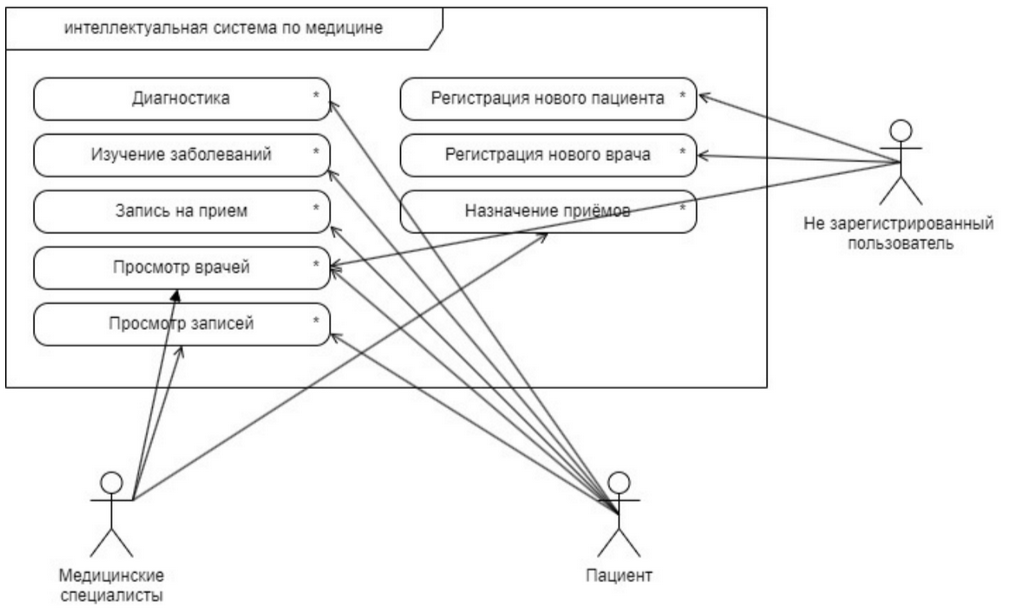
\includegraphics[width=1\textwidth]{sections/users_cases.PNG}
    \caption{Диаграмма использования системы}
    \label{диаграмма использования}
\end{figure}



\subsection{Архитектура системы}

Интеллектуальная система по медицине должна иметь следующую архитектуру:

\begin{itemize}
    \item База знаний данной интеллектуальной системы по медицине.
    \item Решатели задач персонального ассистента по медицине.
    \item Интерфейс персонального ассистента по медицине, представленный в виде веб-приложения.
    \item RAG система для загрузки и обработки медицинских документов, а также созможности составления отчетов по состоянию здоровью пациента
\end{itemize}

\subsubsection{Архитектура базы знаний}
В базе знаний по медицине используется технология OSTIS, а в качестве средства представлений знаний - SC-код и SCg, с помощью которых были формально описаны знания и представлены знания в форме семантической сети.

Основная функция базы знаний для интеллектуальной системы по медицине заключается в обеспечении доступа к надежной и актуальной информации о причинах заболеваний, методах лечения и профилактике. Это позволяет увеличить точность диагностики болезней по заданным симптомам. Данная база знаний также предполагает возможность возможность использования не только для диагностики заболеваний, а также и для получения актуальной и достоверной информации о конкретных заболеваниях.

Интеллектуальная система позволяет пользователям проводить предварительную диагностику заболеваний по конкретным симптомам, а также получать необходимую информацию о запрашиваемом заболевании и рекомендациям по здоровью при данном заболевании. 

База знаний данной интеллектуальной системы включает в себя 6 разделов:
\begin{itemize}
    \item ПрО медицинских процедур;
    \item ПрО медицинских карт;
    \item ПрО медицинской диагностики;
    \item ПрО заболеваний;
    \item ПрО методов лечения;
    \item ПрО организации медицинских учреждений.
\end{itemize}
Данные разделы также в свою очередь делятся на подразделы. Структура базы знаний изображена на рисунке \hyperref[структура базы]{2.2}.
\begin{figure}[H]
  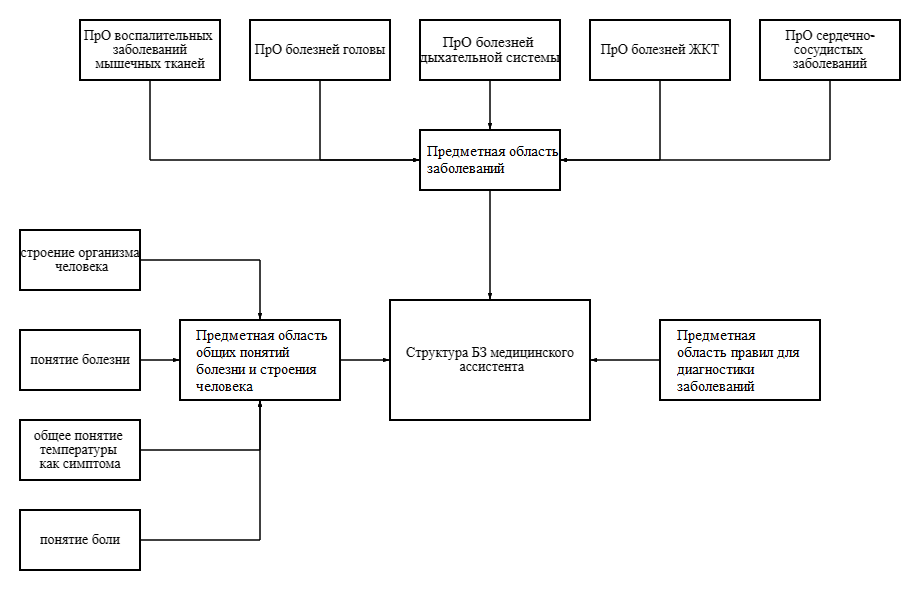
\includegraphics[width=1\textwidth]{sections/diagram (5.1).png}
    \caption{Структура базы знаний}
    \label{структура базы}
\end{figure}

Важной задачей проектирования является интеграция актуальной медицинской информации, что позволит пользователям быстро находить необходимые данные о здоровье. Система будет регулярно обновляться, учитывая последние исследования и практики, что повысит осведомленность пользователей и улучшит качество медицинского обслуживания.


\subsubsection{Архитектура решателей задач}

Основная цель интеллектуальной системы в области медицины заключается в создании эффективного решателя задач, который предоставит пользователям точные и своевременные рекомендации на основе введенного запроса. Решатель задач будет служить центральным компонентом системы, обрабатывающим пользовательские запросы и обеспечивающим доступ к структурированной базе знаний о заболеваниях, их причинах, методах лечения и профилактике, а также предоставлять возможность самостоятельной диагностики диагностики пользователям. Кроме этого решатели задач будут задействованы при прохождении пользователем процедуры регистрации и авторизации в веб-приложении. Исходя из этого обязательными для интеграции в веб-приложение являются следующие агенты-решатели:
\begin{itemize}
    \item агент-решатель задач, предназначенный для регистрации пользователя в интеллектуальной системе.
    \item агент-решатель задач, предназначенный для авторизации пользователя в интеллектуальной системе.
    \item агенты-решатели задач, предназначенные для диагностики заболеваний на основе анализов крови пациента.
    \item агент-решатель задач, предназначенный для навигации пользователя в базе знаний и формирования ссылки с текстом, включающим в себя описание запрашиваемого узла в базе знаний
    \item агент-решатель задач, предназначенный для предоставления рекомендаций по здоровью при определенной болезни для пациента
    \item агент-решатель задач, предназначенный для диагностики предполагаемых заболеваний на основе выбранных симптомов при заполнении формы для диагностики.
\end{itemize}



\subsubsection{Алгоритм работы и принципы разработки агента диагностики по симптомам}
\textbf{Диагностики заболеваний на основе заполнения формы с симптомами.} Для выявления заболевания на основе прохождения пользователем на главной странице веб-приложения формы с указанием симптомов был разработан агент, осуществляющий поиск в базе знаний системы подходящих по симптоматике болезней, а также определяющий предполагаемую вероятность данного заболевания на основе входных данных. Также в рамках работы агента была добавлена возможность поиска как простых симптомов, так и сложных, включающих в себя такие основные отношения, как локализация и характер симптома.

\textbf{Алгоритм работы агента-решателя:}

\begin{enumerate}[label=\arabic*)]
    \item Исходя из результатов заполнения формы для диагностики на главной странице веб-приложения формируется вводная структура, включающая в себя выбранные в форме симптомы.
    \item Используя функции поиска в базе знаний системы для каждого симптома в входной структуре осуществляется поиск и добавление в промежуточный вектор хранения информации название болезни, которой соответствует данный симптом.
    \item Далее на основе подсчета количества вхождений каждой болезни в вектор хранения промежуточной информации формируется пара в виде: болезнь - количество вхождений в вектор. Исходя из принципа работы агенты количество вхождений болезни в промежуточный вектор хранения информации будет соответственно представлять собой количество симптомов из входной структуры, которые соответствуют симптоматике данной болезни.
    \item Формируя в результате своей работы выходную структуру с информацией о болезни и количестве подходящих к ней симптомов агент возвращает данную информацию в веб-приложение, где на основе этих данных определяется вероятность успешной диагностики, ее результаты отображаются в специальном окне и заносятся в историю проводимых диагностик 
\end{enumerate}


\subsubsection{Архитектура веб-приложения}

Для разработки веб-приложения медицинской системы был выбран микросервисный подход. Веб-приложение медицинской системы, разработанное с использованием микросервисного подхода, представляет собой распределённую архитектуру, состоящую из нескольких независимых компонентов. Такое приложение позволяет гибко управлять различными аспектами медицинских данных, упрощает обновления и масштабирование системы. Основные компоненты системы включают в себя:
\begin{itemize}
    \item Клиентский браузер;
    \item веб-сервер;
    \item сервер базы данных;
    \item микросервис для взаимодействия с платформой Ostis;
    \item платформа Ostis.
\end{itemize}
Веб-приложение медицинской системы, состоящее из перечисленных компонентов, структурируется по микросервисной архитектуре, которая организована в несколько ключевых слоев. Такое разбиение упрощает масштабируемость и управление системой, а также улучшает её отказоустойчивость.

Основные слои архитектуры включают:
\begin{itemize}
    \item Клиентский слой – это интерфейс, через который пользователи взаимодействуют с системой. Он представлен в виде клиентского приложения (обычно веб-интерфейса), с которым работают через браузер. На этом уровне реализуются элементы интерфейса пользователя, такие как формы, кнопки, панели, таблицы, и обеспечивается интуитивное взаимодействие с данными. Все запросы, выполняемые с клиентского слоя, направляются на серверную часть системы для обработки, а затем возвращаются в виде ответов или обновлённого интерфейса.
    \item Слой микросервисов (бизнес-логика). На уровне микросервисов располагается основная бизнес-логика приложения. Каждый микросервис является отдельным, независимым компонентом, который может работать автономно, что облегчает разработку и развёртывание. Разделение бизнес-логики на микросервисы позволяет реализовать масштабируемую и устойчивую к сбоям архитектуру: при необходимости можно расширить конкретный сервис без изменения других частей системы.
    \item Слой данных включает в себя сервер базы данных, который хранит и управляет всей медицинской информацией. На этом уровне организуется доступ к данным о пациентах, их истории приёмов, назначениях, записи о медицинских процедурах и других аспектах, необходимых для функционирования системы.
\end{itemize}

Для обеспечения эффективного взаимодействия между архитектурными слоями приложения, каждый из них обращается к функциональности других через API — программный интерфейс, который позволяет компонентам взаимодействовать друг с другом, не зная деталей их внутренней реализации. API стандартизирует обмен данными и вызов функциональных возможностей. Такойподход позволяет каждому компоненту развиваться независимо, так как другие части системы обращаются к нему через установленный интерфейс, не затрагивая внутреннюю логику.

Для создания API в микросервисной архитектуре используется подход REST, который обеспечивает удобный и понятный интерфейс для взаимодействия между клиентом и сервером. RESTful API, благодаря своей гибкости и простоте, является оптимальным выбором для распределённых систем. Он позволяет легко масштабировать приложение, а также организовать обмен данными между независимыми сервисами.

Диаграмма взаимодействия компонентов веб-приложения представлена на рисунке \hyperref[структура приложения]{2.3}.
\begin{figure}[H]
  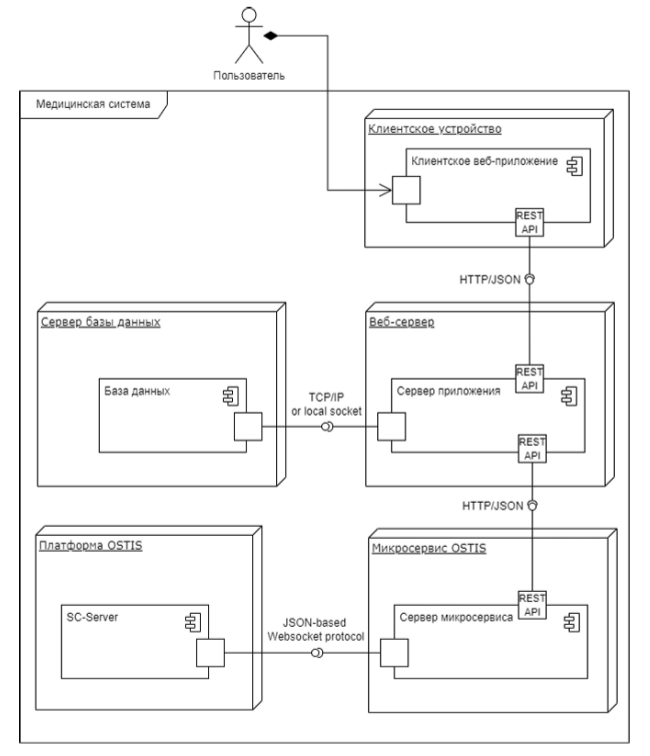
\includegraphics[width=1\textwidth]{sections/web_struct.PNG}
    \caption{Диаграмма взаимодействия компонентов веб-приложения}
    \label{структура приложения}
\end{figure}

\newpage


\subsection{Вывод}
Спроектированная модель медицинского ассистента представляет собой инновационную систему, объединяющую современные технологии и методы медицинского анализа для предоставления персонализированной диагностики. Ассистент будет оснащен функционалом по анализу симптомов, предоставлению диагностических рекомендаций и поддержке в принятии решений как для пациентов, так и для медицинского персонала.

Реализация данной модели имеет потенциал решить множество проблем, с которыми сталкиваются как пациенты, так и медицинские учреждения. Среди основных преимуществ можно выделить:

\begin{itemize}
    \item Оптимизация работы медицинского персонала. Система может обрабатывать большой объем данных и предоставлять врачам ценную информацию для поддержки в принятии решений, что помогает сократить время диагностики и улучшить качество обслуживания пациентов.
    \item Обширность и достоверность информации. Интеллектуальная система содержит подробную и актуальную информацию о различных аспектах здоровья и медицины, проверенную медицинскими экспертами и основанную на научных исследованиях и клинических рекомендациях.
    \item Удобство доступа. Пользователям предоставлен удобный интерфейс для вызова и отслеживания результатов работы вызываемых решателей задач в интеллектуальной системе, а также функционал интеллекутального чата для для быстрых вопросов по истории болезней и рекомендациям по здоровью без привлечения помощи медицинского персонала
    \item Поддержка персонализированных консультаций. Интеллектуальная система предоставляет инструменты самостоятельной диагностики для пользователей.
    \item Наличие страницы личных сообщения для обеспечения оперативной коммуникации между медицинским персоналом и пациентом в режиме реального времени
\end{itemize}

Реализация модели также предполагает обеспечение безопасности и конфиденциальности данных пациентов, а также необходимость непрерывного обновления и адаптации системы в соответствии с изменяющимися потребностями медицинского сообщества.

